% FLOW: research paper.
% Build: cd paper && make   (pdflatex + bibtex; see paper/README.md)
\documentclass[10pt,twocolumn]{article}
\usepackage[T1]{fontenc}
\usepackage[utf8]{inputenc}
\usepackage{lmodern}
\usepackage{textcomp}
\usepackage[margin=0.85in,columnsep=0.3in]{geometry}
\usepackage{microtype}
\usepackage{booktabs}
\usepackage{array}
\usepackage{tabularx}
\usepackage{graphicx}
\usepackage[export]{adjustbox}
\usepackage{xcolor}
\usepackage{listings}
\usepackage{tikz}
\usetikzlibrary{arrows.meta,positioning,calc,fit,backgrounds}
\usepackage{pgfplots}
\pgfplotsset{compat=1.18}
\usepackage[hyphens]{url}
\usepackage[colorlinks=true,linkcolor=black,citecolor=black,urlcolor=black]{hyperref}
\usepackage{enumitem}
\setlist{nosep,leftmargin=1.3em}

% Author line: change here.
\newcommand{\paperauthor}{Nikhil Ajay Kadalge}
\newcommand{\paperaffil}{Independent}
\newcommand{\repo}{\url{https://github.com/nik190799/flow}}
\newcommand{\paperemail}{\href{mailto:nikhil.kadalge@gmail.com}{nikhil.kadalge@gmail.com}}
\newcommand{\paperorcid}{ORCID: \href{https://orcid.org/0009-0004-8859-5607}{0009-0004-8859-5607}}
\newcommand{\paperdoi}{DOI: \href{https://doi.org/10.5281/zenodo.24411135}{10.5281/zenodo.24411135}}

\lstset{basicstyle=\ttfamily\footnotesize,breaklines=true,columns=fullflexible,
  frame=single,framerule=0.3pt,rulecolor=\color{black!40},xleftmargin=2pt,xrightmargin=2pt,
  aboveskip=6pt,belowskip=4pt,showstringspaces=false}
\newcommand{\code}[1]{\texttt{#1}}
\usepackage{xspace}
\newcommand{\ms}{\,ms\xspace}
\newcommand{\s}{\,s\xspace}
\renewcommand{\arraystretch}{1.08}
\sloppy

\title{\textbf{FLOW: Functions as Live Overlays, Without Restart.\\[2pt]
\large An Architecture for Applications That People and Their Agents Change While They Run}}
\author{\paperauthor\\{\small \paperaffil}\\{\small\paperemail \quad \paperorcid}\\{\small\repo \quad \paperdoi}}
\date{November 2026 \quad (v0 preprint)}

\begin{document}
\maketitle

\begin{abstract}
The Live Layer Protocol (LLP) lets signed WebAssembly code replace parts of a running application
without a restart and without losing state. It does not say \emph{who} may change \emph{which}
part of an application, or what a change may do with a person's data. FLOW is an architecture on
top of LLP that answers those questions. A company ships a \emph{core} and declares two things
about it: labelled \emph{data} (public, personal, secret) and \emph{directions}, the places where
people's own \emph{functions} may run and what they may read and use. A person, or an AI agent
holding a time-limited \emph{grant} from that person, signs a function into a direction. The device
alone decides: it checks every signature against a root-signed keyring whose root includes a
quantum-safe (SLH-DSA) key group, refuses before any code runs a function whose declared reads and
capabilities could carry personal data off the device, runs functions as overlays that a company
release can never be blocked by, and lets the person undo any function, restoring its old code
\emph{and} its old data across a change of data format. A fixed table of element meanings lets the
same function appear as a web page, terminal text, speech, or a tool list for an agent. We report a
JavaScript implementation wired to the unchanged LLP host (185 checks pass), a second verifier in Go
that passes the same 40 frozen conformance vectors, and a seven-line ``bar'' run side by side
against an ordinary web application: the web application fails six lines and partly passes one,
FLOW passes all seven. On one 4-vCPU machine a signed release swaps in 4.2\ms (median of 15), a
person's function installs in 3.0\ms and is undone in 1.1\ms. With 200 functions running, a company
release still lands in 13--15\ms, but the reference host spends about 11\,MB per function, which
rules out cheap devices today. We close with a thesis, labelled as such: applications are turning
into \emph{data plugins} that bring their data and primitives while the system draws the interface
on demand. We cite the platform moves that point that way, show the idea running on a calculator,
and argue that the missing half of that future is the trust model FLOW provides.
\end{abstract}

\section{Introduction}

Today a company ships an application and every user gets the same one. If a person wants it to work
differently, they ask the company, wait for a release, or work around it with a browser extension
or user script that the next release silently breaks. Two trends make this arrangement look old.
First, code is cheap: a language model writes a small function from one sentence in seconds, so
the person who wants the change can often have it written for them. Second, the code that would
make the change can now be delivered into a running program safely: the Live Layer Protocol
(LLP)~\cite{llp2026} streams small signed WebAssembly~\cite{haas2017wasm} modules into a running
application, rehearses them on a copy of the real state, swaps them in milliseconds, and reverts
them when they fail.

What is missing is an architecture that says who may change what. LLP trusts one publisher key per
application. It has no notion of a person changing their own copy, of an AI agent acting for a
person, of which data a piece of code may see or send, or of how a company's release and a person's
change coexist. Without those answers the safe options are the two we already have: nobody but the
company changes the application, or anyone does, through extensions that can read everything on
the page~\cite{kapravelos2014hulk}.

FLOW (\emph{Functions as Live Overlays, Without restart}) is that architecture. Its position is
that an application should be a \emph{core} owned by a company plus \emph{overlays} owned by
whoever is accountable for them, and that every decision about what runs is made by the
\emph{device}, from signatures and declarations it can check, never by a server.

\paragraph{Contributions.}
\begin{enumerate}
\item A model of who changes a running application: four layers (owner, backend, device, user) and
five change paths (\S\ref{sec:model}).
\item The FLOW design (\S\ref{sec:a1}--\ref{sec:b1}): a signed envelope and a keyring trust policy
with quantum-safe root keys and rotation that cannot be stripped or forged; directions, data labels
and a declared-flow rule; people's functions as overlays with undo across data-format changes;
grants for AI agents; and a fixed table of element meanings for many surfaces.
\item A JavaScript implementation on the unchanged LLP host, a Go verifier, 40 frozen conformance
vectors, and a reference application (\S\ref{sec:impl}).
\item An evaluation (\S\ref{sec:eval}): a seven-line bar run against an ordinary web application,
security proofs, costs, and a 200-function scale run that exposes a real memory limit.
\item A thesis, with cited evidence and a running example, that applications are becoming data
plugins whose interfaces the system draws on demand (\S\ref{sec:thesis}).
\end{enumerate}

\paragraph{Scope and honesty.} FLOW is at revision B1 and has no production deployment. Every
number in this paper was produced by a script in the repository and re-run for this paper on one
cloud VM (\S\ref{sec:setup}); the raw output is in \code{paper/results/}. Section~\ref{sec:thesis}
is a forward-looking argument, not a result: the sources it cites describe platform features, and
the conclusion we draw from them is ours.

\section{Background: the Live Layer Protocol}
\label{sec:llp}

LLP~\cite{llp2026} delivers code as \emph{layers}: WebAssembly modules identified by the SHA-256 of
their bytes. A signed, monotonic \emph{manifest} maps named \emph{slots} to layer hashes. A
\emph{Live Host} owns all application state as a key/value store, so replacing code cannot lose it.
On a new manifest the host checks the signature and version, fetches missing layers by hash, opens
a copy-on-write shadow of state, loads each changed layer, runs its migration hook and one render on
the shadow, and commits all slots or none. Each later call is a transaction with time and memory
limits; a layer that traps is reverted to the newest earlier version whose data schema matches.
A manifest may restrict each slot to the state keys it owns and reads and to the capabilities
(haptics, network, \ldots) it may request. Layers return a small tree of UI elements, which the host
draws. These mechanisms descend from dynamic software updating~\cite{hicks2005dsu} and Erlang's
release handling~\cite{armstrong2003}; LLP's contribution is to verify each change at the moment it
arrives at the running program, against that program's real state.

FLOW uses LLP as a library at a pinned commit and changes none of its code.

\section{Who Changes a Running Application}
\label{sec:model}

We model a live application as four layers.
\begin{enumerate}
\item \textbf{Owner}: the company. It holds the signing keys and decides which parts of the
application users may change.
\item \textbf{Backend}: relays changes and stores shared and per-user data. It can carry a change
but can never sign or approve one.
\item \textbf{Device}: runs the host, verifies every signature, and hot-swaps code while keeping
state. Nobody overrides it.
\item \textbf{User}: a person, who usually directs an AI agent rather than writing code.
\end{enumerate}
A change travels by one of five paths (Figure~\ref{fig:paths}): \textbf{A}, the owner to every
device through the backend; \textbf{B}, a user's change to everyone, only if the owner signs it;
\textbf{C}, a user's change to their own devices through the backend; \textbf{D}, a user's change on
one device with no backend; \textbf{E}, device to device with no backend (a file, a QR code, a local
network). User changes sit on top of the owner's application, only where the owner opened it, and
can always be rolled back.

\begin{figure}[t]
\centering
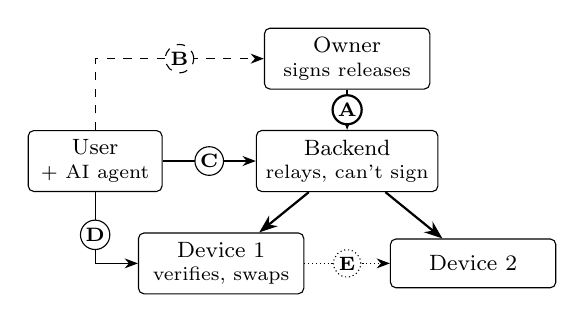
\begin{tikzpicture}[font=\footnotesize,>=Stealth,
  box/.style={draw,rounded corners=2pt,minimum width=2.1cm,minimum height=0.62cm,align=center},
  lab/.style={circle,draw,fill=white,inner sep=0.8pt,font=\scriptsize\bfseries}]
  \node[box] (O) at (0.6,2.6) {Owner\\[-1pt]{\scriptsize signs releases}};
  \node[box] (B) at (0.6,1.3) {Backend\\[-1pt]{\scriptsize relays, can't sign}};
  \node[box,minimum width=1.7cm] (U) at (-2.6,1.3) {User\\[-1pt]{\scriptsize + AI agent}};
  \node[box] (D1) at (-1.0,0) {Device 1\\[-1pt]{\scriptsize verifies, swaps}};
  \node[box] (D2) at (2.2,0) {Device 2};
  \draw[->,thick] (O) -- node[lab]{A} (B);
  \draw[->,thick] (B) -- (D1); \draw[->,thick] (B) -- (D2);
  \draw[->,dashed] (U.north) |- node[lab,pos=.75]{B} (O.west);
  \draw[->] (U) -- node[lab]{C} (B);
  \draw[->] (U.south) |- node[lab,pos=.3]{D} (D1.west);
  \draw[->,densely dotted] (D1) -- node[lab]{E} (D2);
\end{tikzpicture}
\caption{The four layers and five change paths. B needs the owner's signature. The backend carries
changes on A and C but cannot sign them.}
\label{fig:paths}
\end{figure}

The model asks more of the device than LLP does. The device must know whose signature counts for
which document, which parts of the application a user may touch, what data may leave, and how a
user's change survives the owner's next release. FLOW is the answer to those questions. Revision
A1 (\S\ref{sec:a1}) makes trust a policy rather than a key; revision B1 (\S\ref{sec:b1}) adds people's
functions. Table~\ref{tab:paths} states which paths exist today.

\begin{table}[t]
\centering\footnotesize
\begin{tabularx}{\columnwidth}{@{}lX@{}}
\toprule
Path & Status in revision B1 \\
\midrule
A & Built: signed releases under the keyring's release policy. \\
B & Not built. A person's function never reaches another device. \\
C & Not built. Functions stay on the device they were installed on. \\
D & Built: people's and agents' functions, signed on the device. \\
E & Partly: releases and keyrings install from a folder of files with no network; functions do not
travel this way yet. \\
\bottomrule
\end{tabularx}
\caption{The five paths and what revision B1 implements.}
\label{tab:paths}
\end{table}

\section{Revision A1: Trust as a Policy}
\label{sec:a1}

A1 is the groundwork that is cheap before devices are in the field and costly after: once a device
trusts only today's key type, it cannot be taught to trust a stronger one without a signature it
can already verify.

\subsection{The envelope}

Every signed FLOW document travels in one wrapper:
\begin{lstlisting}
{ "flow": 1, "type": "flow/keyring",
  "payload": "<base64url>",
  "sigs": [{ "kid": "sha256:...", "sig": "..." }] }
\end{lstlisting}
Each signature covers
\code{"FLOWv1" SP len(type) SP type SP len(payload) SP payload}, the DSSE pre-authentication
encoding~\cite{dsse} with a FLOW prefix. Because the document \emph{type} is signed, a keyring
signature cannot be presented as a release signature. Because the wrapper is not signed, reformatting
it changes nothing, and verifiers must ignore wrapper fields they do not know. Signatures are counted
over the raw payload \emph{before} it is parsed. The payload must be valid UTF-8 JSON with no key
repeated within an object, since parsers disagree on which copy of a repeated key wins and such a
document could mean different things on different hosts.

\subsection{Signature suites}

A1 defines two suites: \code{p256} (ECDSA over P-256 with SHA-256, as in LLP) and
\code{slh-dsa-sha2-128s} (SLH-DSA, FIPS~205~\cite{fips205}), a hash-based scheme believed to resist
quantum attack. A key's id is \code{sha256} over the suite name, a zero byte and the public key, so
an id names exactly one key of one suite. Signatures in suites a verifier does not implement are
ignored rather than fatal; whether they were needed is the policy's question.

\subsection{The keyring}

A \code{flow/keyring} document lists keys and, per role, groups of keys, each with a threshold.
\textbf{A document is valid for a role only if every group of that role meets its threshold}, and a
key that signs twice counts once. The \code{root} role must include at least one quantum-safe group
from the first keyring on (otherwise \code{weak\_root}). A keyring also commits, by id, to one spare
root key that is not active.

A device at keyring $N$ accepts keyring $M$ only if $M$ is signed under the full root policy of
$N$ (the committed spare may stand in for one lost key, revealing its public key, which must hash to
the committed id), $M$ is well formed, is for the same application, has a higher number, and is
signed under its own full root policy; if the spare was used, $M$ must commit to a new one. So an
attacker who cannot satisfy today's policy cannot change it; an attacker holding keys of one suite
cannot strip the other; and the root can still deliberately add, replace or retire a suite. This is
the TUF~\cite{samuel2010tuf} and Uptane~\cite{kuppusamy2016uptane} idea of threshold-signed,
self-rotating roles, applied with a mandatory post-quantum group. Trust comes only from the keyring
on the device, never from what a document says about itself. The first keyring ships with the host
or is pinned by hash at install.

\subsection{Releases, tolerance, time and old engines}

A \code{flow/release} carries an LLP manifest and must meet the keyring's \code{release} role.
FLOW documents follow one tolerance rule: unknown fields are ignored, and anything a host must
understand is named in \code{requires}; a host lacking a named feature refuses with
\code{host\_too\_old} instead of guessing. A device that has no trustworthy clock is told so
(\code{clock: "untrusted"}) and then decides by signatures and rising numbers alone. A host may
require every layer to use only the 2017 WebAssembly~1.0 feature set (the reference host does by
default) so that old engines can run it. Keyrings, a release and its layers can be installed from a
folder of files, with every file going through the same checks. The 40 test vectors written the day
A1 was frozen are locked by hash; every later revision must keep passing them.

\section{Revision B1: People's Functions}
\label{sec:b1}

B1 is what makes a FLOW application more than an application that updates itself. It changes none
of A1.

\subsection{What a release declares}

A release may carry four more fields:
\begin{lstlisting}
"data": { "jobs.": "personal",
          "catalog.": "public", "vault.": "secret" },
"capabilities": { "upload": { "egress": true },
                  "haptic": { "egress": false } },
"core": ["main"],
"directions": { "side": { "read": ["jobs."],
   "caps": ["haptic"], "egress": "public",
   "max": 4, "after": "main" } }
\end{lstlisting}
\code{data} labels state-key prefixes. Data nobody labelled counts as personal, and keys under
\code{fn/} (people's functions' own data) are always personal. \code{capabilities} says which
capabilities can carry data off the device (\code{egress}) and how sensitive their results are; an
undescribed capability is assumed to leave the device. A \textbf{direction} is a named spot where
people's functions may run: the prefixes a function there may read, the capabilities it may ask for,
the most sensitive data that may leave through it, how many functions it holds, and where they are
shown. A direction may never offer secret data.

\subsection{The declared-flow rule}

For any code, its \emph{sensitivity} is the most sensitive label among what it may read and what its
capabilities return; its \emph{ways out} are its capabilities with egress. Code whose sensitivity is
personal or secret must have no way out, unless it is in the company's \code{core} (the company
answers for its own application) or, for a function, its direction allows personal data out
\emph{and} the person agreed on the device. This is a two-point instance of lattice-based information
flow~\cite{denning1976lattice}, checked at install time over \emph{declarations}, not values: it does
not trace data through the code, as language-based systems do~\cite{myers1997dlm}. Code that is
allowed both personal data and a way out is trusted with it, which is why that combination needs
both the company's ceiling and the person's consent. Panel reviewers of an earlier FLOW design
found that access control alone was not enough: a function that may read personal data and also
use the network leaks it through its own output. The flow rule is the answer.

\subsection{Functions}

A \code{flow/function} names the application, a direction, an id, a rising \code{seq}, the layer's
hash, its reads and capabilities, and a stated intent. It is signed by a person enrolled on the
device, or by an agent whose grant travels beside it. Before fetching or running any of its code,
the host checks eight rules (Figure~\ref{fig:install}): a valid signer, the right application, an
open direction, reads and capabilities within the direction, the flow rule, consent where needed, a
higher \code{seq} than any version this device ever accepted (so an undone version cannot be
replayed), and room in the direction. Only then is the layer fetched, checked by hash and against
WebAssembly~1.0, and rehearsed on real state like any LLP layer.

\begin{figure}[t]
\centering
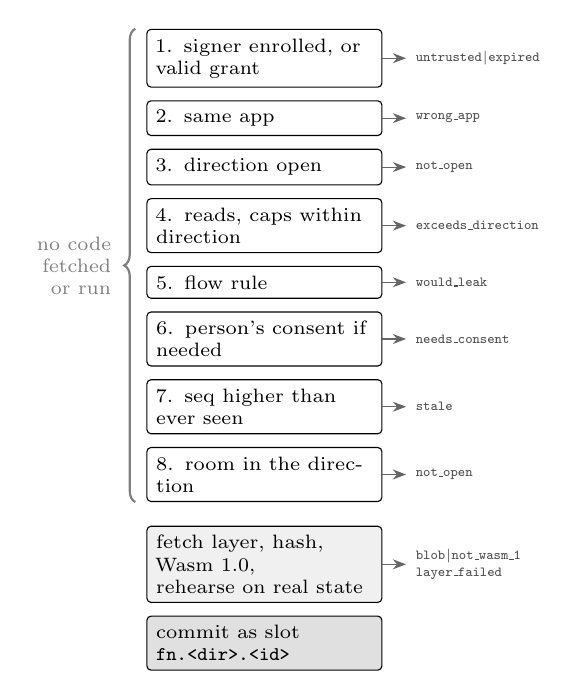
\begin{tikzpicture}[font=\scriptsize,>=Stealth,node distance=0.16cm,
  st/.style={draw,rounded corners=1.5pt,minimum height=0.36cm,align=left,text width=2.75cm},
  no/.style={font=\tiny\ttfamily,text=black!70,anchor=west,align=left}]
  \node[st] (s1) {1. signer enrolled, or valid grant};
  \node[st,below=of s1] (s2) {2. same app};
  \node[st,below=of s2] (s3) {3. direction open};
  \node[st,below=of s3] (s4) {4. reads, caps within direction};
  \node[st,below=of s4] (s5) {5. flow rule};
  \node[st,below=of s5] (s6) {6. person's consent if needed};
  \node[st,below=of s6] (s7) {7. seq higher than ever seen};
  \node[st,below=of s7] (s8) {8. room in the direction};
  \node[st,below=0.3cm of s8,fill=black!6] (s9) {fetch layer, hash, Wasm 1.0,\\rehearse on real state};
  \node[st,below=of s9,fill=black!12] (s10) {commit as slot \code{fn.<dir>.<id>}};
  \foreach \i/\c in {1/untrusted\textbar expired,2/wrong\_app,3/not\_open,4/exceeds\_direction,5/would\_leak,6/needs\_consent,7/stale,8/not\_open} {
    \draw[->,black!60] (s\i.east) -- ++(0.3,0) node[no]{\c};
  }
  \draw[->,black!60] (s9.east) -- ++(0.3,0) node[no]{blob\textbar not\_wasm\_1\\layer\_failed};
  \draw[decorate,decoration={brace,amplitude=4pt,mirror},thick,black!50] ([xshift=-4pt]s1.north west) -- ([xshift=-4pt]s8.south west)
    node[midway,left=5pt,align=right,font=\scriptsize]{no code\\fetched\\or run};
\end{tikzpicture}
\caption{Installing a person's function. Every refusal carries a code an agent can act on.}
\label{fig:install}
\end{figure}

A running function lives in slot \code{fn.<direction>.<id>}. It owns the keys under
\code{fn/<direction>/<id>/} and can write nothing else; it can read only its own keys and its declared
prefixes; any other capability call is refused at run time. A text field it shows may be bound only
to a key it owns, and a presenter must not show it a value it cannot read.

\subsection{Overlays: releases and functions never block each other}

Installing, updating, undoing or removing a function never restarts the company's slots. When a
company release is accepted, each installed function is checked again; one that no longer fits (its
direction closed, a prefix withdrawn, a ceiling lowered) is \textbf{paused}: its code stops, its data
stays, and the release goes ahead. It runs again when a later release fits it. A function whose code
fails is paused, its failed write dropped, and the rest of the application carries on. \emph{A
function cannot stop a release from being accepted.}

\subsection{The person's controls and agents' grants}

\textbf{Undo} puts back the previous version of a function \emph{and} that function's own data as it
was just before the update, including the stored schema number, so undo works across a change of
data format. \textbf{Remove} deletes the function and everything under its keys. Both are local acts
that need no signature, network or company.

A \code{flow/grant}, signed by an enrolled person, lets an agent's key sign functions for listed
directions until a time limit, optionally for a subset of capabilities. A grant only narrows: the
function must still pass every rule as if the person signed it, and the person is recorded as
answering for it. This is the caveated, attenuating delegation of macaroons~\cite{birgisson2014macaroons}
and object capabilities~\cite{miller2006robust}, kept local to the device. A device without a
trustworthy clock refuses all grants, because their point is the time limit. The device keeps a
record of every accepted change: release keys, the signing key, the accountable person, the grant,
the stated intent, and every undo, pause and enrolment.

\subsection{Elements: one function, many surfaces}

A layer's view is a tree of elements. B1 fixes the meaning of each kind (group, heading, text, text
field, button, switch) as a role, a name, a state and an action, in the spirit of
WAI-ARIA~\cite{wcagaria}; an unknown kind is a group, so a newer element still shows its contents on
an older host. The host ships four presenters that read this one table: a web page, terminal text,
speech, and a tool list for an agent, in which the tools are exactly the buttons and switches on
screen and a text field that submits to a button is that tool's input. An agent can therefore do
through a function exactly what the person can do by hand, and nothing more. The page presenter
patches the page in place and reads typed text from the host's live value, so focus, caret and
half-typed text survive a swap of the code behind them without the author doing anything.

\section{Implementation}
\label{sec:impl}

The JavaScript implementation is 1{,}428 lines (\code{src/}): envelope, suites, keyring, the
WebAssembly~1.0 checker, functions and the flow rule, \code{FlowHost}, and the four presenters. It
depends on LLP at a pinned commit and on \code{@noble/post-quantum} for SLH-DSA. It has no
Node-only code and runs in a browser page as well. The Go verifier (557 lines,
\code{go/flow}) implements A1 with Cloudflare's CIRCL for SLH-DSA.

\paragraph{The bridge.} The LLP host verifies an LLP signature on every manifest and fails closed
without one. \code{FlowHost} creates a key that exists only in its own process and gives the LLP host
the \emph{effective manifest}: the company's manifest plus one slot per running function, with each
function's keys and capabilities fenced as in \S\ref{sec:b1}. It signs that manifest with the bridge
key only after every FLOW check passed (Figure~\ref{fig:bridge}). No LLP safety check is switched off,
and nothing FLOW refused can reach the LLP host. The LLP host sees a private rising counter as the
version; FLOW applies LLP's replay rules to the company's own $(\mathit{epoch},\mathit{version})$.

\begin{figure}[t]
\centering
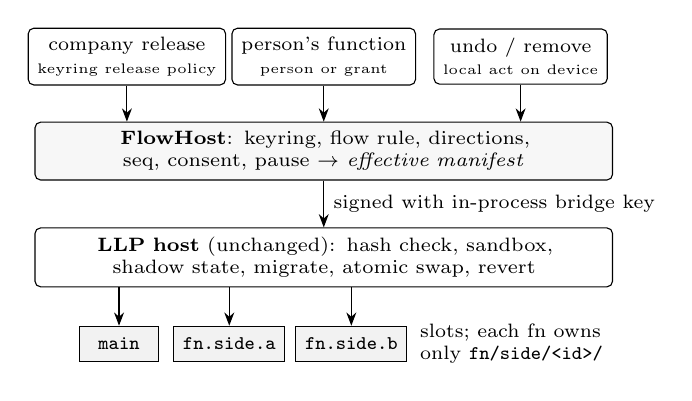
\begin{tikzpicture}[font=\scriptsize,>=Stealth,
  b/.style={draw,rounded corners=2pt,align=center,minimum height=0.55cm},
  s/.style={draw,fill=black!5,minimum width=1.0cm,minimum height=0.45cm,font=\scriptsize\ttfamily}]
  \node[b,minimum width=2.2cm] (rel) at (-2.5,1.7) {company release\\{\tiny keyring release policy}};
  \node[b,minimum width=2.2cm] (fn) at (0.0,1.7) {person's function\\{\tiny person or grant}};
  \node[b,minimum width=2.2cm] (undo) at (2.5,1.7) {undo / remove\\{\tiny local act on device}};
  \node[b,text width=7.1cm,fill=black!3] (fh) at (0,0.5) {\textbf{FlowHost}: keyring, flow rule, directions, seq, consent, pause $\rightarrow$ \emph{effective manifest}};
  \draw[->] (rel) -- (rel|-fh.north); \draw[->] (fn) -- (fn|-fh.north); \draw[->] (undo) -- (undo|-fh.north);
  \node[b,text width=7.1cm] (llp) at (0,-0.85) {\textbf{LLP host} (unchanged): hash check, sandbox, shadow state, migrate, atomic swap, revert};
  \draw[->] (fh) -- node[right]{signed with in-process bridge key} (llp);
  \node[s] (m) at (-2.6,-1.95) {main};
  \node[s] (f1) at (-1.2,-1.95) {fn.side.a};
  \node[s] (f2) at (0.35,-1.95) {fn.side.b};
  \node[font=\scriptsize,align=left,anchor=west] at (1.1,-1.95) {slots; each fn owns\\only \code{fn/side/<id>/}};
  \draw[->] (llp.south) ++(-2.6,0) -- (m.north); \draw[->] (llp.south) ++(-1.2,0) -- (f1.north); \draw[->] (llp.south) ++(0.35,0) -- (f2.north);
\end{tikzpicture}
\caption{FLOW over LLP. FLOW decides; LLP executes the effective manifest exactly as it executes any manifest.}
\label{fig:bridge}
\end{figure}

\paragraph{Reference application.} \code{examples/workorders} is a field-service application: a
company work-order list, a person's own van checklist in a \code{side} direction, an agent's
``next up'' function under a ten-minute grant, a function that would upload customer addresses
(refused), and a forged release (refused), all drawn by FLOW's page presenter. A Chromium test
presses the same buttons a visitor would (10 of 10 checks pass).

\section{Evaluation}
\label{sec:eval}

\subsection{Setup}
\label{sec:setup}

One cloud VM: 4 vCPU (Intel Xeon, 2.30\,GHz), 15.7\,GiB RAM, Linux, Node~22.23.5, Go~1.25.0,
Chromium through Playwright. All runs were made on 21 November 2026 at repository commit
\code{d30c329} plus the \code{paper/} directory. Timings are wall-clock on a shared VM; we report
medians and ranges where we repeated runs, and say so where a number comes from a single run.

\subsection{Tests and conformance}

\code{npm test} runs 185 checks, all passing, in 49\s (most of it SLH-DSA signing in pure
JavaScript): 26 unit checks, 18 WebAssembly~1.0 checks (including agreement with wabt on all 34 LLP
and FLOW layers), 25 proofs, 13 LLP-host integration checks, 51 function checks, 8 presenter checks,
4 offline-install checks and the 40 frozen vectors. The Go verifier passes its unit tests and the
same 40 vectors, so two independent verifiers return the same refusal code for every vector.

Table~\ref{tab:proofs} lists the safety properties the proofs establish by running them.

\begin{table}[t]
\centering\footnotesize
\begin{tabularx}{\columnwidth}{@{}Xl@{}}
\toprule
Property (each run as a test) & Result \\
\midrule
Release with the SLH-DSA or the P-256 signature stripped & refused \\
Keyring change signed only by new keys, or only by old & refused \\
All root keys replaced, signed under old and new policy & accepted \\
Attacker with one P-256 root key adds a release key & refused \\
Keyring 2 signed with classical root keys only & refused \\
Keyring 2 that drops the quantum-safe root group & refused \\
Lose one root key; rotate with the remaining ones & accepted \\
2-of-2 SLH-DSA root, one key lost, spare revealed & accepted \\
Spare whose public key doesn't match the commitment & refused \\
Documents with invented fields (incl.\ a sensitivity label) & accepted \\
Requires a feature the host lacks & \code{host\_too\_old} \\
Release signed outside the keyring reaches LLP & never \\
Layer using bulk memory (post-1.0) & \code{not\_wasm\_1} \\
Install from files with no network; tampered file & ok; refused \\
\bottomrule
\end{tabularx}
\caption{A1 proofs (from \code{test/proofs.mjs}, \code{test/host.mjs}, \code{test/offline.mjs}).}
\label{tab:proofs}
\end{table}

\subsection{The bar}

To check that a FLOW application is more than an application that updates itself, we wrote seven
lines that an ordinary application cannot pass and test them side by side: the same small task
application built as an ordinary web application (run in Chromium, with a server that can swap its
script) and as a FLOW application (run in Node and in Chromium). Table~\ref{tab:bar} gives the
results of \code{npm run bar}.

\begin{table}[t]
\centering\footnotesize
\begin{tabularx}{\columnwidth}{@{}lXcc@{}}
\toprule
\# & Line & Web app & FLOW \\
\midrule
1 & Changed while in use, nothing lost & fail & pass \\
2 & Each person's copy differs, yet stays the company's app & fail & pass \\
3 & The device has the last word & fail & pass$^{a}$ \\
4 & Every change has a named signer and a working undo & fail & pass \\
5 & A function touches only what it declared & fail & pass$^{b}$ \\
6 & It works with no network & fail & pass \\
7 & One function, many surfaces & partial & pass \\
\bottomrule
\end{tabularx}
\caption{The bar. $^{a}$For an installed host; when the checker is itself a web page, whoever serves
the page can replace it. $^{b}$Judged on declarations, not traced values.}
\label{tab:bar}
\end{table}

What the lines found, briefly. (1)~In Chromium a signed release swapped the running code in 4.2\ms
while the person was mid-word; the field kept its text, focus and caret and was the same DOM node,
in this run and 8 of 8 more. With the presenter's live-text fix switched off, typed text was lost in
6 of 10 runs, a gap that also existed in LLP's own web demo and was fixed there. The web application
showed no change until a reload, which lost the half-typed text. (2)~A user script on the web
application starred two tasks; after the company renamed one CSS class it starred none, silently.
In FLOW, a person's function signed by her own key installed in 2\ms beside the company's code,
another person's device on the same release refused it, a company update left it running, and
closing the direction paused it with its data kept. (3)~Acting as a hostile server we tried five
ways to push code or trust into FLOW (relay-signed release, swapped layer, edited release, new
keyring, replayed old release); all were refused and the application kept running. The web
application ran the hostile script on the next load and sent the tasks out. (4)~The company undid
a release in the open application in 1.6\ms; the person undid her own function in 1.2\ms, getting
back old code and old data across a format change. (5)~The web user script declared nothing and
sent all stored data off the device; in FLOW a function declaring ``read tasks'' plus ``network'' was
refused before any of its code ran. (6)~With the network removed, a new keyring and release installed
from files. (7)~One unchanged function was shown as a page, as terminal text, as speech, and as two
agent actions that an agent then used.

\subsection{Costs}

\begin{table}[t]
\centering\footnotesize
\setlength{\tabcolsep}{4pt}\begin{tabular}{@{}lrrr@{}}
\toprule
Suite & Sign (p50) & Verify (p50) & Signature \\
\midrule
P-256 (WebCrypto) & 0.25\ms & 0.20\ms & 64\,B \\
SLH-DSA-128s (JS) & 1{,}210\ms & 1.51\ms & 7{,}856\,B \\
\bottomrule
\end{tabular}
\caption{Signature cost (\code{paper/bench-crypto.mjs}; P-256 $n{=}200$, SLH-DSA sign $n{=}7$,
verify $n{=}30$). An envelope with one signature of each suite is 10{,}817\,B as JSON.}
\label{tab:crypto}
\end{table}

\paragraph{Signatures.} Table~\ref{tab:crypto}. Verifying the quantum-safe signature costs a device
about 1.5\ms; signing costs the author about 1.2\s in pure JavaScript, which is acceptable for root
keys that sign rarely and is why A1 uses SLH-DSA only for the root role. Releases are signed with
P-256 today; ML-DSA~\cite{fips204} release keys can be added by an ordinary keyring change when
maintained libraries exist on both host platforms.

\paragraph{Swap, install, undo.} Over 15 runs of the integration tests, a FLOW release (envelope and
keyring check, then LLP's verified swap) swapped the running layer in a median 4.2\ms (range
2.7--7.8); a person's function installed in a median 3.0\ms (2.3--7.9); and undo across a data-format
change took a median 1.1\ms (0.7--1.5).

\paragraph{Scale.} The architecture plan asked whether a device can hold 50 and 200 functions. We
installed $N$ functions across four directions, then shipped a company release and undid one
function with all $N$ running (\code{paper/bench-scale.mjs}; Table~\ref{tab:scale}). Correctness
held: every release landed and every function kept running. Latency stayed small. Memory did not:
the reference LLP host runs each layer instance in its own worker thread, and the process grew by
about 11\,MB per function, to 2.3\,GB at 200 (the same when 200 ran alone). That is acceptable on a
desktop and rules out the cheap tablets this design is meant to reach. Running many small functions
in one engine instance, or one worker per direction, is the obvious fix and is not built.

\begin{table}[t]
\centering\footnotesize
\begin{tabular}{@{}rrrrrr@{}}
\toprule
$N$ & Install p50 & Release & Undo & Render & RSS \\
\midrule
1 & 3.9\ms & 26.4\ms$^{a}$ & 1.1\ms & 0.3\ms & 80\,MB \\
10 & 25.4\ms & 4.1\ms & 1.7\ms & 0.8\ms & 188\,MB \\
50 & 18.3\ms & 14.7\ms & 4.5\ms & 2.9\ms & 619\,MB \\
200 & 19.6\ms & 14.7\ms & 10.9\ms & 7.1\ms & 2{,}284\,MB \\
\bottomrule
\end{tabular}
\caption{$N$ people's functions on one device (single run each; a second run of 50 and of 200 in
fresh processes gave 6.2/12.7\ms releases and 623/2{,}272\,MB). $^{a}$The first run in the process
pays for cold workers.}
\label{tab:scale}
\end{table}

\section{Thesis: Applications as Data Plugins}
\label{sec:thesis}

\emph{This section is an argument about where software is heading. It is not a result of this paper.
The platform features we cite exist; the conclusion we draw from them is our own extrapolation, and
none of the cited sources claims it.}

\subsection{The claim}

We argue that applications are turning into \textbf{data plugins}. An application will increasingly
bring three things to a person's device: its \emph{data} (and the live sources it pulls data from),
its \emph{primitives} (the operations it knows how to perform on that data, its own interpretation
of it), and its \emph{rules} (who may build on it, with what, and where results may go). The
interface will increasingly be drawn by the system the person is using (an operating system, an
assistant, an agent host), for the need and context of the moment, rather than shipped as a fixed
set of screens. New functions will be composed on demand, by the person or by an agent working for
them, out of those primitives. The goal is not that software is controlled remotely, but that it
\emph{adapts} to the people using it: to their context and to the way they think.

\subsection{Evidence that platforms are moving this way}

Table~\ref{tab:evidence} lists recent platform moves. They split into two halves. In the first,
applications expose functions and data to the system instead of only to their own screens. In the
second, the system or an agent generates the interface.

\begin{table*}[t]
\centering\footnotesize
\begin{tabularx}{\textwidth}{@{}llXc@{}}
\toprule
When & Who & What it does & Half \\
\midrule
May 2025 & Microsoft~\cite{windowsmcp2025} & Native MCP support in Windows: ``a standardized framework for AI agents to connect with native Windows apps''; apps wrap features as MCP servers in an OS registry; agent access off by default. & functions \\
Nov 2025 & MCP maintainers, OpenAI, Anthropic~\cite{mcpapps2025,sep1865} & MCP Apps: servers ``deliver interactive user interfaces to hosts'' in sandboxed iframes; the authors note it ``is starting to look like an agentic app runtime''. & UI \\
Nov 2025 & Google Research~\cite{googlegenui2025} & Generative UI: the model generates ``an entire user experience'' per prompt; in evaluation, people preferred it nearly as often as expert-made sites and well above other formats; generation ``can sometimes take a minute or more''. & UI \\
Dec 2025 & Google~\cite{a2ui2025,newstack2025} & A2UI: agents send ``a declarative data format, not executable code'', a tree of components from a catalog the client trusts, to ``generate the interface which best suits the current conversation''. & UI \\
Feb 2026 & Google (Android)~\cite{intelligentos2026} & ``The Intelligent OS'': AppFunctions let apps ``expose data and functionality directly to AI agents''; success shifts from opening the app to fulfilling the user's task. & functions \\
2026 & Google (Android)~\cite{appfunctions} & AppFunctions: apps ``behave like on-device MCP servers'' registered with the OS, replacing ``step-by-step, manual navigation'' through the app's UI. & functions \\
2026 & Apple~\cite{appleintents} & App Intents: Apple Intelligence ``combines language models with your app's actions and content''; apps declare intents, entities and enumerations to the system. & functions \\
\bottomrule
\end{tabularx}
\caption{Platform moves toward applications as function and data providers (left half) and
system-generated interfaces (right half). Quotations are from the cited pages.}
\label{tab:evidence}
\end{table*}

The idea is not new; what is new is a capable generator. OpenDoc~\cite{apple1996opendoc} tried to
replace applications with parts embedded in one document. Naked Objects~\cite{pawson2004naked}
generated the whole interface from domain objects. The Personal Universal Controller generated remote
controls for appliances from a description of their functions~\cite{nichols2002puc}, and
SUPPLE~\cite{gajos2004supple} generated interfaces optimised for a device and a person's abilities.
These systems showed that an interface can be derived from functions and data; they lacked a
generator able to handle open-ended needs, and they lacked the incentive of platforms wanting agents
to reach into applications. Language models now supply the first, and the moves in
Table~\ref{tab:evidence} show the second.

\subsection{The calculator}

Take a calculator. It brings data (the number on the display) and primitives (the digits 0--9, the
operators $+$, $-$, $\times$, $\div$, and sine and cosine). Everything else a person might want is a
composition of those, and today the person gets only the compositions the vendor drew buttons for.
In the data-plugin view the vendor ships the data and primitives and opens a direction; the person
asks for what they need and gets a function \emph{and its interface} on demand.

We built this on FLOW and ran it (\code{paper/calculator/}, 12 of 12 checks). The company's release
is a core slot \code{pad} owning \code{calc.} (labelled personal) and one direction:
\begin{lstlisting}
"directions": { "fx": { "read": ["calc."],
  "caps": [], "egress": "none", "after": "pad" } }
\end{lstlisting}
The company's \code{sin} works in radians. Ana wants degrees; she signs a function that reads
\code{calc.x} and draws its own panel (installed in 4.5\ms, no company signature, no restart; it shows
$\sin 30^\circ = 0.5$). An agent, under Ana's ten-minute grant, adds a bill splitter with its own text
field, button and tip switch, interfaces the company never drew (31\ms, recorded as Ana's
responsibility). The agent then drives it through the declared actions: \code{go(How many people)},
\code{tip}; 120 between 4 with tip is 34.5 each. A function asking for the network is refused before
it runs (\code{exceeds\_direction}). The company ships release~2, adding $\surd$ and \%, in 7.3\ms; both
functions keep running and follow the number ($\surd 144 = 12$, $\sin 12^\circ = 0.207912$). Ana undoes
the agent's function in 2\ms, and after ten minutes the agent can change nothing. Figure~\ref{fig:calc}
shows the result as drawn by FLOW's page presenter; the same functions read aloud as ``Split 120 +
15\% tip between 4. Each pays 34.5. Text field: How many people, contains 4. Button: Split. Switch, on:
Add 15\% tip.''

\begin{figure*}[t]
\centering
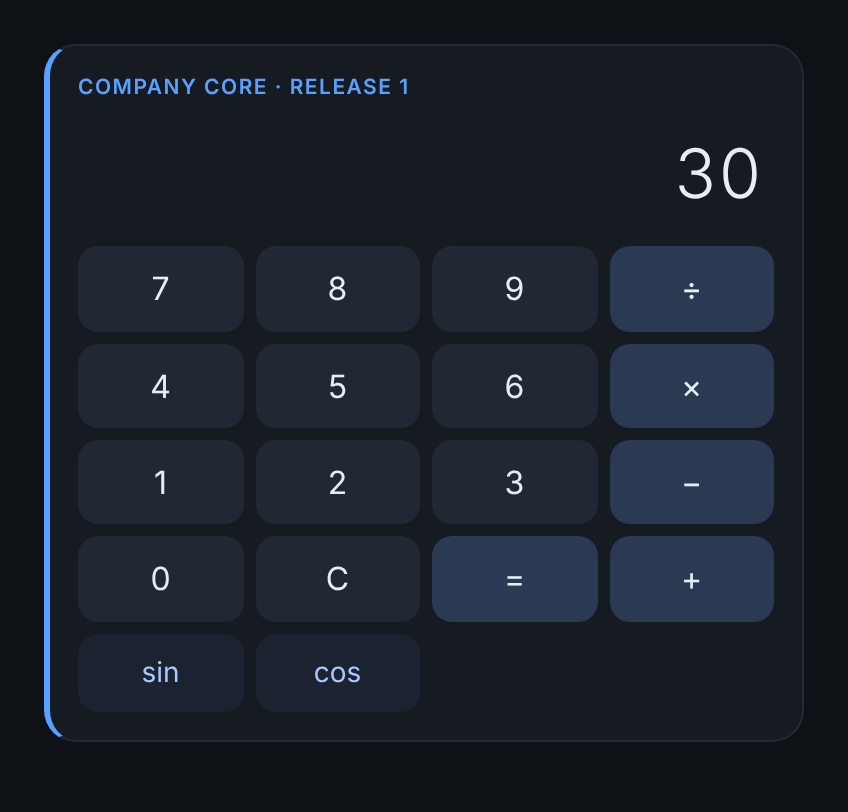
\includegraphics[width=0.28\textwidth,valign=t]{figures/calc-1.png}\quad
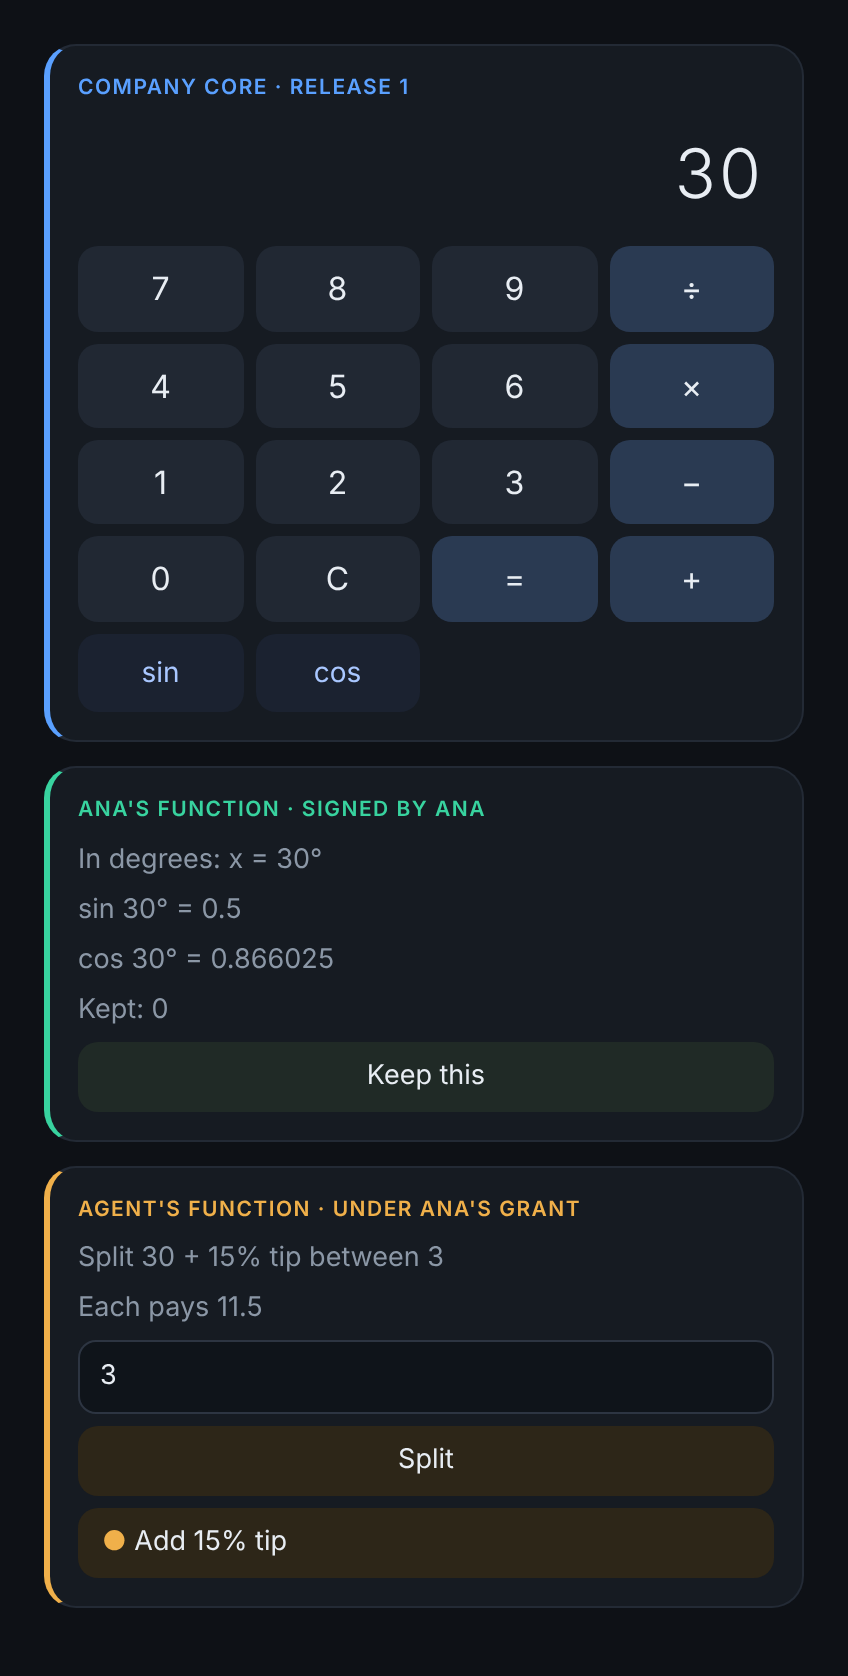
\includegraphics[width=0.28\textwidth,valign=t]{figures/calc-2.png}\quad
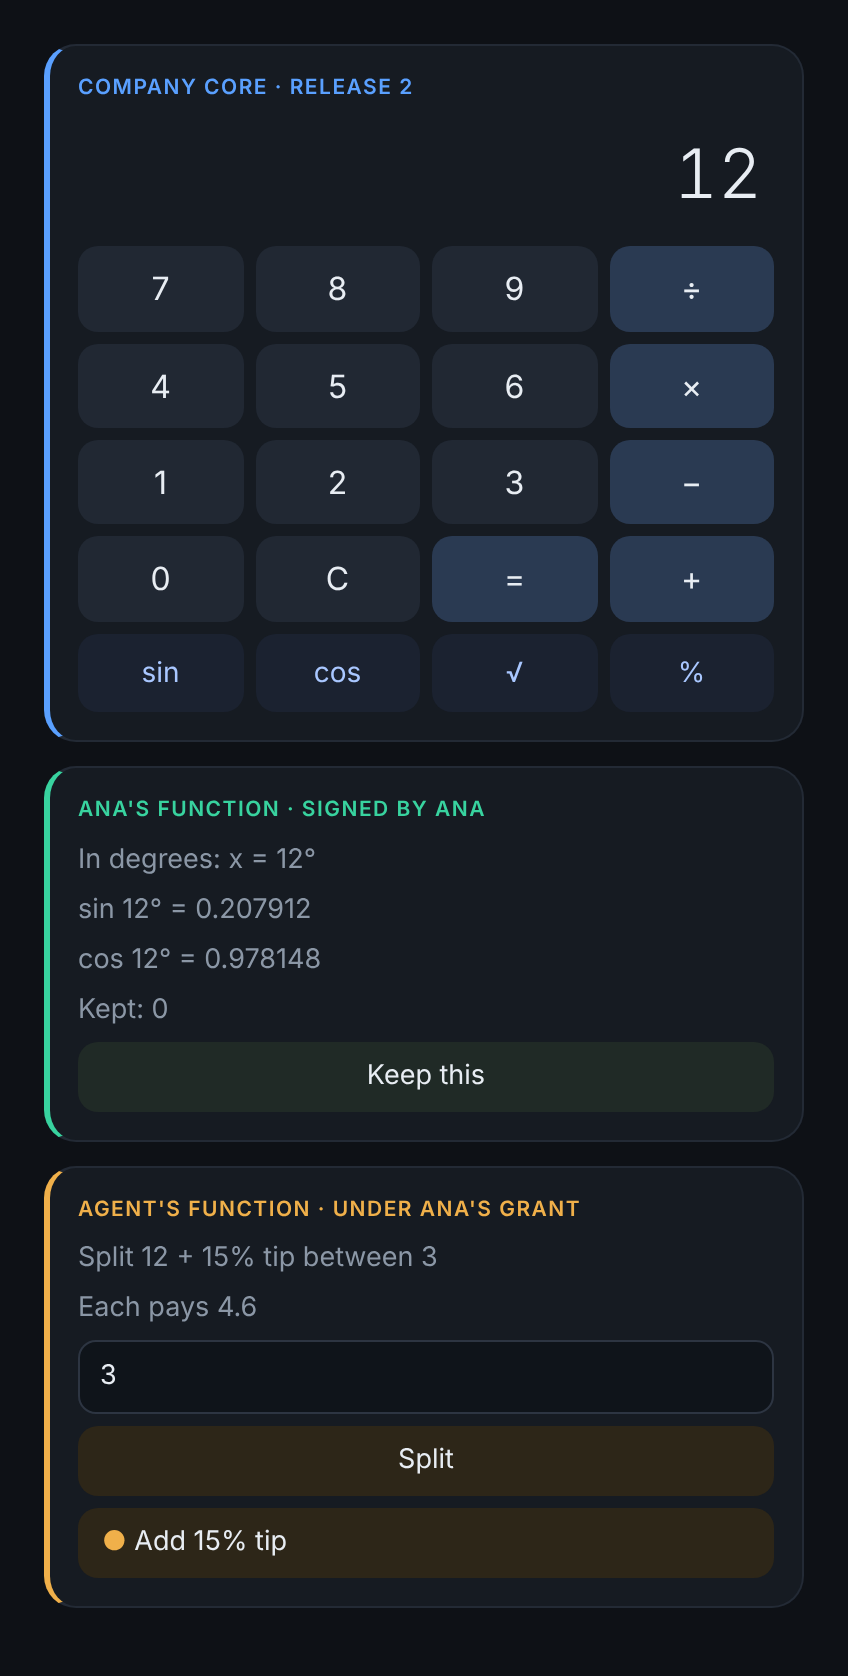
\includegraphics[width=0.28\textwidth,valign=t]{figures/calc-3.png}
\caption{The calculator as a data plugin, drawn by FLOW's page presenter from the element tree each
layer returns (styling is the page's CSS). Left: the company's release~1 alone. Middle: Ana's degrees
function (signed by Ana) and an agent's bill splitter (under Ana's grant), added on demand beside the
core. Right: the company's release~2 adds $\surd$ and \% while both functions keep running and follow
the number. Captured by \code{paper/calculator/figure.mjs}.}
\label{fig:calc}
\end{figure*}

In this example the layers still describe their own element trees; the system's part is to present
them on any surface and to let an agent use them. The thesis goes further: the person's system would
generate the function's code and view from the request. FLOW does not do that generation, and
generated code is exactly what it is built to receive.

\subsection{What the trend is missing}

The sources in Table~\ref{tab:evidence} make applications callable and interfaces generatable. They
say little about four questions that become urgent once interfaces and functions are produced on
demand, often by an agent and often unwatched: \emph{Who answers for this code?} \emph{What data may it
carry off the device?} \emph{Can the person take it back?} \emph{Does it survive the vendor's next
update?} Current answers are sandboxing (MCP Apps' iframes), a declarative catalog that ships no
code (A2UI), and permissions that ask the person, which people often do not attend
to~\cite{felt2012permissions}.

FLOW offers one consistent answer, and we argue it is the trust half of the data-plugin future:
every function is signed by a person or by an agent under that person's grant (accountability); data
carries labels and directions carry ceilings, checked before code runs (flow); undo restores code and
data on the device (reversibility); and functions are overlays that a vendor release pauses rather
than breaks (coexistence). A2UI's trusted component catalog and FLOW's fixed element table are the
same idea from two sides: the system, not the generated code, owns what an element means.

\subsection{Predictions, and what would refute the thesis}

If the thesis holds, we expect: (1)~every major operating system to expose a registry in which
applications declare functions and data for agents (Android, Windows and Apple platforms have
begun); (2)~a semantic, declarative interface format, rather than pixels or arbitrary code, to become
the common way agents put interfaces in front of people; (3)~platforms to add identity, delegation
and data-flow rules for generated code, rather than relying only on per-call permission prompts.
The thesis would be weakened if people reject generated interfaces in favour of fixed applications
once the novelty fades, if generation latency (a minute or more today~\cite{googlegenui2025}) does
not fall to interactive levels, or if platforms keep application data closed to third-party agents.

\section{Related Work}

\paragraph{Live update.} Dynamic software updating~\cite{hicks2005dsu}, Erlang
releases~\cite{armstrong2003} and LLP~\cite{llp2026} change running code; mobile over-the-air update
services~\cite{expoupdates} ship company code without store review. None of them lets a person add
code beside the company's, or reasons about whose code may see what.

\paragraph{Update security.} TUF~\cite{samuel2010tuf}, Uptane~\cite{kuppusamy2016uptane} and
Sigstore~\cite{newman2022sigstore} establish who may sign a release and how to recover from key
loss; DSSE~\cite{dsse} defines the signed envelope FLOW adapts. FLOW's keyring follows TUF's
threshold, self-rotating roles and adds a mandatory quantum-safe root group~\cite{fips205} from the
first keyring, because a device cannot later be taught to trust a stronger key type without a
signature it already trusts.

\paragraph{Information flow and capabilities.} The flow rule is a coarse, install-time application of
Denning's lattice model~\cite{denning1976lattice}; decentralized label models~\cite{myers1997dlm}
track values through code, which FLOW does not. Grants follow attenuating delegation
\cite{birgisson2014macaroons,miller2006robust}.

\paragraph{Extensions and malleable software.} Browser extensions and user scripts let people change
applications, but with broad access and no stable extension points~\cite{kapravelos2014hulk}.
Malleable-software research argues people should be able to reshape their tools~\cite{litt2025malleable};
Webstrates~\cite{klokmose2015webstrates} makes documents and applications shareable, editable media;
local-first software~\cite{kleppmann2019localfirst} puts the person's device and data first. FLOW
shares these goals and adds the company's side: declared directions, labels and a signed core that
people's changes overlay but cannot break.

\paragraph{Plugin runtimes.} WebAssembly plugin frameworks~\cite{extism} and the component
model~\cite{componentmodel} provide sandboxed, typed extension, typically installed by the host
application's author. FLOW is about who may install which extension, and what it may do with data.

\section{Limitations}
\label{sec:limits}

\begin{itemize}
\item \textbf{Paths B, C and E for functions are not built} (Table~\ref{tab:paths}); a person's
functions live on the device they were installed on.
\item \textbf{Nothing persists across a host restart.} People, functions, grants and the record live
in memory.
\item \textbf{The flow rule is declared, not traced.} Code allowed both personal data and a way out is
trusted with it.
\item \textbf{One implementation of B1.} The Go verifier and the frozen vectors cover A1 only.
\item \textbf{No cost budgets.} The plan's rule that every function declares what it may cost the
device, and never delays the next frame, is not built; only LLP's per-call time and memory limits apply.
\item \textbf{Memory per function.} About 11\,MB each in the reference host (Table~\ref{tab:scale}).
\item \textbf{Releases are signed with P-256}; the quantum-safe group protects the root, not yet each
release.
\item \textbf{A web-page host can be replaced by whoever serves the page}; the device's last word holds
for an installed host.
\item \textbf{Small element set}: no lists, images or navigation yet. \textbf{The first keyring} is
trusted by shipping or by pin, not by signature.
\item \textbf{Single-machine evaluation}, no field deployment, and no user study of the consent and
undo design.
\end{itemize}

\section{Conclusion}

LLP made it possible to change a running application safely. FLOW makes it possible for the right
people to do so: the company for its core, a person for their own copy, an agent only under a
person's grant, each signature checked by the device against a policy that a server cannot forge and
a quantum attacker cannot strip, each function fenced by what it declared and undoable on the spot.
It passes seven tests an ordinary application cannot, at millisecond cost, with memory per function
as the clearest problem left. We have argued that this is the trust layer that a world of
applications as data plugins, with interfaces drawn on demand, will need.

\paragraph{Availability.} Code, specification (\code{SPEC-A1.md}, \code{SPEC-B1.md}), tests, the
benchmark scripts, the calculator example and the raw results for this paper are at \repo, under
the Apache-2.0 licence.

\bibliographystyle{plain}
\bibliography{refs}

\end{document}
